\documentclass[12pt]{exam}
\usepackage[utf8]{inputenc}
\usepackage[margin=1in]{geometry}
\usepackage{amsmath,amssymb}
\usepackage{multicol}
\usepackage{url}
\usepackage{graphicx}
\usepackage{float}


\PassOptionsToPackage{hyphens}{url}\usepackage{hyperref}
\newcommand{\class}{Robot Intelligence}
\newcommand{\term}{Fall 2022}
\newcommand{\examnum}{Midterm Exam}
\newcommand{\examdate}{8/31/2022}
\newcommand{\timelimit}{10/28/2022}

\pagestyle{head}
\firstpageheader{}{}{}
\runningheader{\class}{\examnum\ - Page \thepage\ of \numpages}{\examdate}
\runningheadrule


\begin{document}

\noindent
\begin{tabular*}{\textwidth}{l @{\extracolsep{\fill}} r @{\extracolsep{6pt}} l}
\textbf{\class} & \textbf{Name:} & \makebox[2in]{\hrulefill}\\
\textbf{\term} &&\\
\textbf{\examnum} &&\\
\textbf{\examdate} &&\\
\textbf{Take Home Exam - Due Before Class on Canvas \timelimit} 
\end{tabular*}\\
\rule[2ex]{\textwidth}{2pt}

This exam contains \numpages\ pages (including this cover page) and \numquestions\ questions.\\
The total number of points is \numpoints. Graduate students must answer some additional questions. Undergraduates answering graduate questions will be given additional points and a feeling of satisfaction from attempting difficult things (probably). 

Any programming/code artifacts associated with this exam should be submitted along with the final PDF to canvas. Please put your entire submission in a single .zip file. 

This exam will cover topics in motion, planning, sensor processing, and ethics.


\begin{center}
    Grade Table (Quick view to see the breakdown)\\
    \addpoints
    \gradetable[v][questions]
\end{center}

\noindent
\rule[2ex]{\textwidth}{2pt}

\begin{questions}

\newpage

\addpoints
\question[20]
    Moving in a car 

   I would like you to use a skid steer model of a robot that is $75cm$ long and $55cm$ wide and run a few simple experiments with it. Please upload your resulting figures and python (or other) code: 
    
\noaddpoints
\begin{parts}
    \part[5] 
        Make a list of commands (at t=0.1) that will allow this robot to traverse along the edge of a $5m$ diameter circle. The robot starts off in the center of the circle (0,0), and you cannot leave the circle's border. Plot both the resulting path (x, y) and trajectory (x, y, and angular velocities). Assume a constant velocity of $8 m/s$
    \part[5]
        Do the same as the above for a traditional car (Ackermann steering). 
    \part[10]
        Your Ackermann vehicle (with the same dimensions as described for the skid steer), is driving on a circle of radius 2.5m. Assume that you begin on the edge of the circle. Calculate the positional error with our computational approximation using the forward Euler method, as referred to in the course notes and illustrated in Reading 2, eq. 1.6. Graph the errors and computing time for three different time-steps ($\Delta t = 1, 0.1, 0.01$), error is defined as the absolute distance between the expected (from equations) to real $x,y$ position (defined analytically) over time.

        Brief notes on what this problem is about: Imagine that you are moving a semi-truck and you have GPS positions (somewhat accurate) and an internal prediction model. We want the internal models to be updated based on "ground truth" information to build better estimates of the vehicle motion over time. 
        
        
        % If the car is traveling for $10s$, what is my position error using the discretized equations of motion if I define my time steps at $\Delta t = 1, 0.1, 0.01$ ? Plot the errors and computing time for the Ackermann vehicle in these cases. Use the forward Euler approach and compute a total error based on the distance difference from the analytical circle to the discrete-time equations. 
    
    \part[10] 
        \textbf{Graduate Student Question} Compute part c again where road frictions are much lower (due to rain or ice). Slip causes your tires to respond very differently. Assume that your theta is $\theta_{actual} = \theta (1 - 0.08)$ and velocity is $v_{actual} = v (1 - 0.04)$.
    \\
    
    \textit{Response:} 
    
    Please run MidtermQ1.py included with this document. It will display all necessary output for parts a) through c). Code used for this problem is also located in MidtermQ1.py
\end{parts}
\newpage


\addpoints
\question[20]
    Inverse Kinematics, numerical approaches
    
    The following SCARA-type manipulator has physical characteristics as follows: 
    $l_1 = 60cm$, $l_2 = 40cm$, and an arbitrary height (ie: assume that $(0,0)$ is at the first motor). 
    
\noaddpoints
\begin{parts}
    \part[5] 
        \begin{figure}
            \centering
            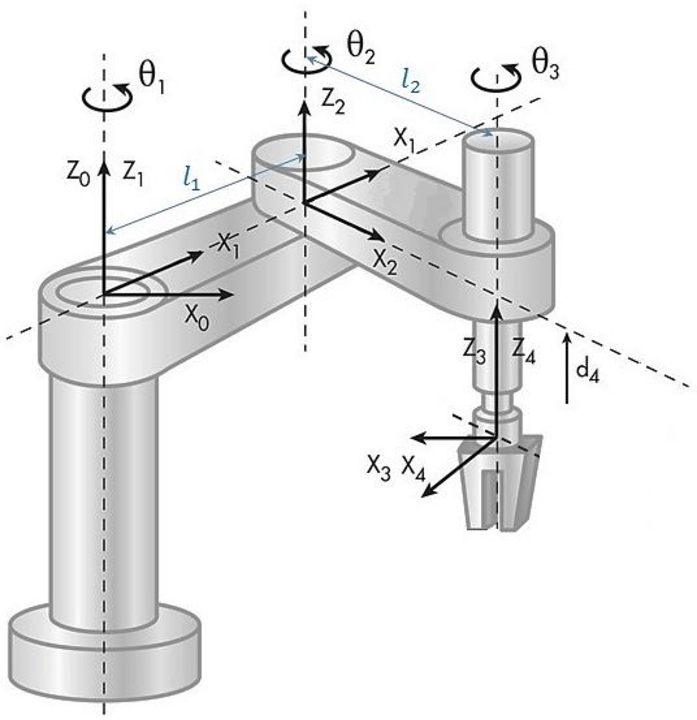
\includegraphics[width=0.5\textwidth]{SCARA-robot-of-4-gdl-Source-Our-elaboration.png}
            \caption{SCARA type manipulator. }
        \end{figure}
        
        What is the workspace volume for this robot?. (Draw a picture of it as well)
        \\\\
        \textit{Response:} 

        The workspace volume is a cylinder with radius 100cm and height h, and there is a cylindrical hole in the center with radius 20cm and height h.

        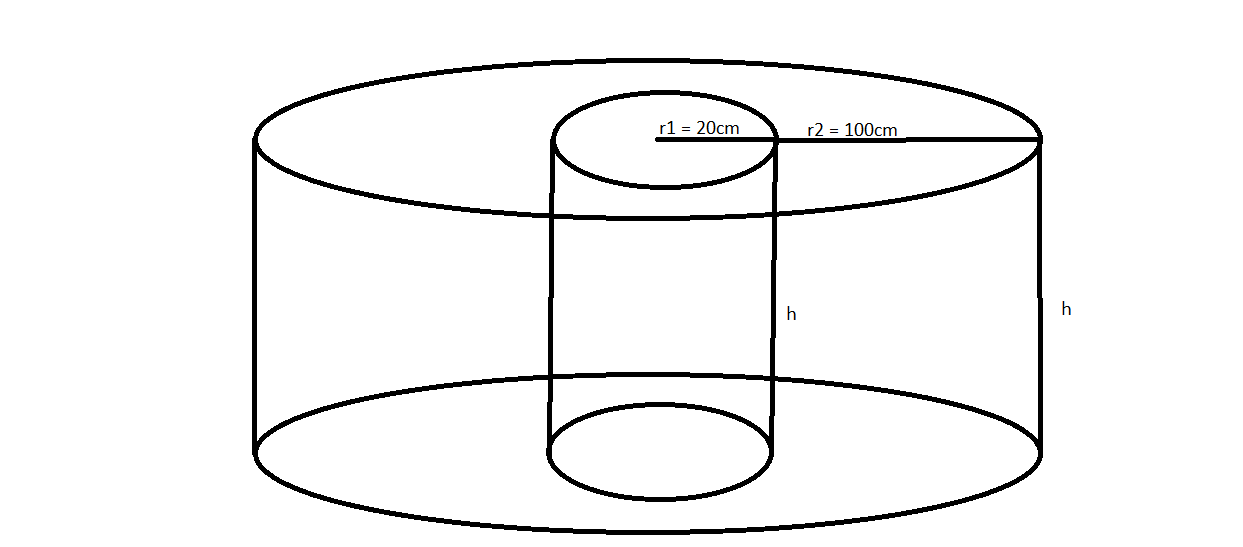
\includegraphics[width=0.5\textwidth]{workspace-volume.png}
        
    
    \part[5] 
        Write the DH parameters 
        \\\\
        \textit{Response:}

        \begin{center}
            \begin{tabular}{ |c|c|c|c|c| } 
             \hline
             Link & $a_i$ & $\alpha_i$ & $d_i$ & $\theta_i$ \\ 
             \hline
             1 & $a_1$ & 0 & 0 & $\theta_1^*$ \\ 
             \hline
             2 & $a_2$ & 0 & 0 & $\theta_2^*$ \\ 
             \hline
             3 & $a_3$ & 0 & $d_3^*$ & $\theta_3^*$ \\
             \hline
            \end{tabular}
            \\
            Note: * = variable
        \end{center}
    
    \part[10] 
        Compute the forward kinematics to find the position of the end effector if $\theta_1 = 30 deg$, $\theta_2 = 45 deg$, $\theta_3 = 90 deg$, and $d = 14 cm$
        \\\\
        \textit{Response:}
        \begin{center}
            \[
                A_1 =
                \begin{bmatrix}
                    c_1 & -s_1 & 0 & a_1c_1 \\
                    s_1 & c_1 & 0 & a_1s_1 \\
                    0 & 0 & 1 & 0 \\
                    0 & 0 & 0 & 1 \\
                \end{bmatrix}
            \]
            \[
                A_2 =
                \begin{bmatrix}
                    c_2 & -s_2 & 0 & a_2c_2 \\
                    s_2 & c_2 & 0 & a_2s_2 \\
                    0 & 0 & 1 & 0 \\
                    0 & 0 & 0 & 1 \\
                \end{bmatrix}
            \]
            \[
                A_3 =
                \begin{bmatrix}
                    c_3 & -s_3 & 0 & a_3c_3 \\
                    s_3 & c_3 & 0 & a_3s_3 \\
                    0 & 0 & 1 & d_3 \\
                    0 & 0 & 0 & 1 \\
                \end{bmatrix}
            \]
            \[
                A_1A_2 =
                \begin{bmatrix}
                    c_{12} & -s_{12} & 0 & a_1c_1 + a_2c_{12} \\
                    s_{12} & c_{12} & 0 & a_1c_1 + a_2s_{12} \\
                    0 & 0 & 1 & 0 \\
                    0 & 0 & 0 & 1 \\
                \end{bmatrix}
            \]
            \[
                A_1A_2A_3 =
                \begin{bmatrix}
                    c_{123} & -s_{123} & 0 & a_3c_{123} + a_1c_1 + a_2c_{12} \\
                    s_{123} & c_{123} & 0 & a_3s_{123} + a_1s_1 + a_2s_{12} \\
                    0 & 0 & 1 & d_3 \\
                    0 & 0 & 0 & 1 \\
                \end{bmatrix}
            \]
            \vspace{5mm} \\
            Equations for coordinates of the end-effector in the base frame:
            \\
            \begin{align}
                x = a_3c_{123} + a_1c_1 + a_2c_{12} \\
                y = a_3s_{123} + a_1s_1 + a_2s_{12} \\
                z = d_3
            \end{align}
            \\
        \end{center}
        If $\theta_1 = 30\deg$, $\theta_2 = 45\deg$, $\theta_3 = 90\deg$, $d_3 = 14 cm$, $a_1 = 60 cm$, $a_2 = 40 cm$, and $a_3 = 0 cm$, the coordinates are:
        \\
        \begin{center}
           $x \approx 62.3 cm$ \\
           $y \approx 68.6 cm$ \\
           $z = 14cm$
        \end{center}
        
\end{parts}
\newpage


\addpoints
\question[20]
    Inverse Kinematics with numerical approaches (Use the manipulator on the following page). Note that $d_6$ refers to the length of the arm on the top and $d_1$ is the length of the system from the base to the first motor.)
    
    
\noaddpoints
\begin{parts}

    \part[10] 
        Compute the joint angles and extension distances that will get this robot to pick up an object at x=1.2, y=0.8, z=0.5 if the robot started at if the robot started with the end effector at $\theta_1= -90deg$, $d_2 = 0.5m$, $d_3 = 1.0m$, $\theta_4=-90deg$, $\theta_5 = 90deg$, $\theta_6 = 40deg$, $d_6 = 0.2m$. Note that $d_6$ is a constant value and that $\theta_6$ will not impact the final solution for our purposes, you are allowed to set $d_1$ as it only impacts the final z position.
        \begin{figure}
        \centering
        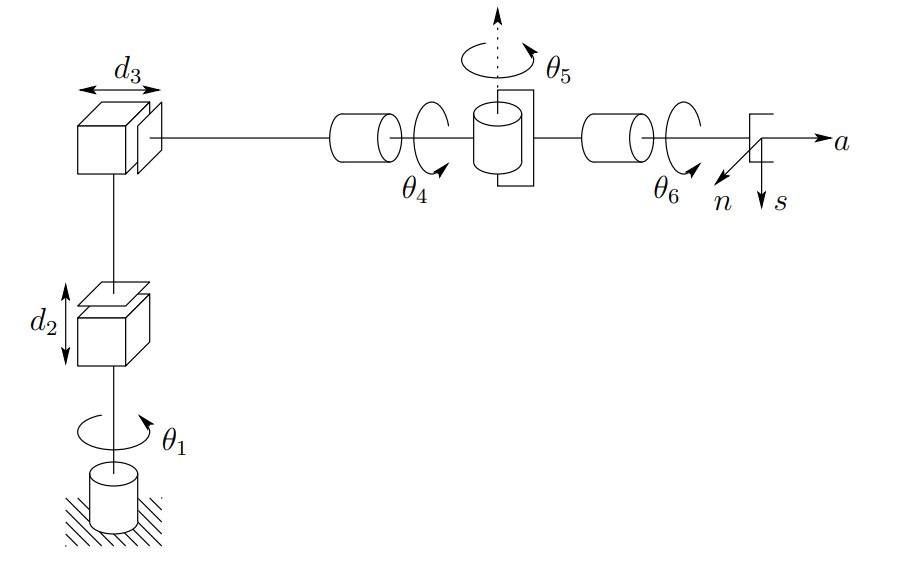
\includegraphics[width=0.5\textwidth]{6dof_arm.jpg}
        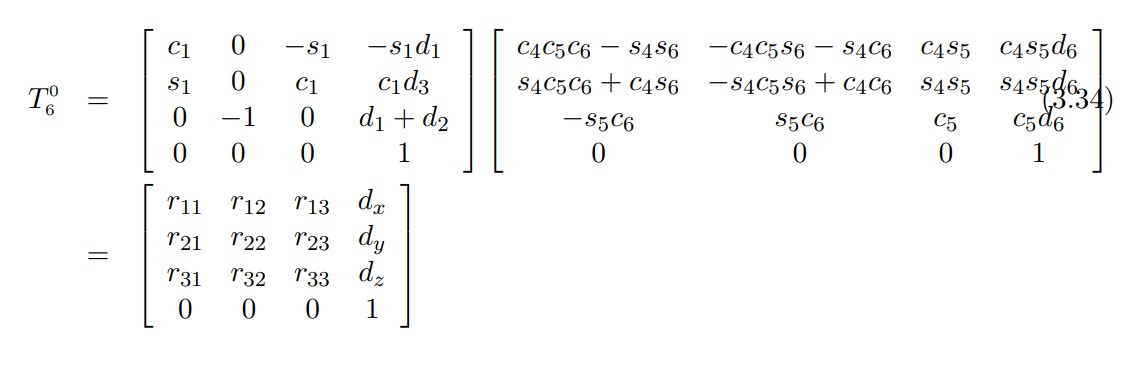
\includegraphics[]{6dof_arm_TMatrix.jpg}
        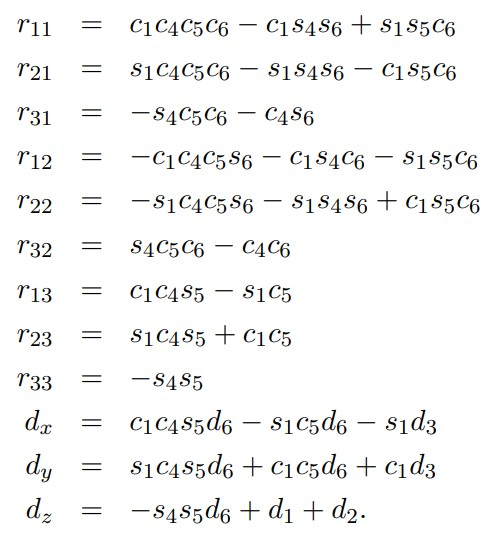
\includegraphics[]{6dof_arm_TMatrix_Eqs.jpg}
        \caption{Cylindrical/Prismatic manipulator. Use for problem 6.}
        \end{figure}
    
    \part[10] 
        What would be the joint angles and extension distances to get to the same goal coordinates if the robot started with the end effector at $\theta_1= 0deg$, $d_2 = 0.2m$, $d_3 = 0.3m$, $\theta_4=-90deg$, $\theta_5 = 90deg$, $\theta_6 = 40deg$, $d_6 = 0.2m$ and we wished to minimize the total distance traveled for each actuating part?
    
    \part[10]
        \textbf{Graduate Question:} Using the same system, start configuration, and goal coordinates of Part B, compute the energy-efficient joint angles and extension distances. For your energy model, assume that actuating $\theta_1$ costs 3x the energy of $\theta_{4,5,6}$, and $d_{2,3}$ costs 2x the energy.
    \\
    
    \textit{Response:} 
    
    Please run MidtermQ3.py included with this document. It will display all necessary output for parts a) and b). Code used for this problem is also located in MidtermQ3.py
    

\end{parts}
\newpage


\addpoints
\question[20]
    Balancing a Pole 
    
    A cart and pole suddenly appear before you, and you feel compelled to answer burning questions you have always held about these systems. 

\noaddpoints
\begin{parts}
    \part[5] 
        \begin{figure}
            \centering
            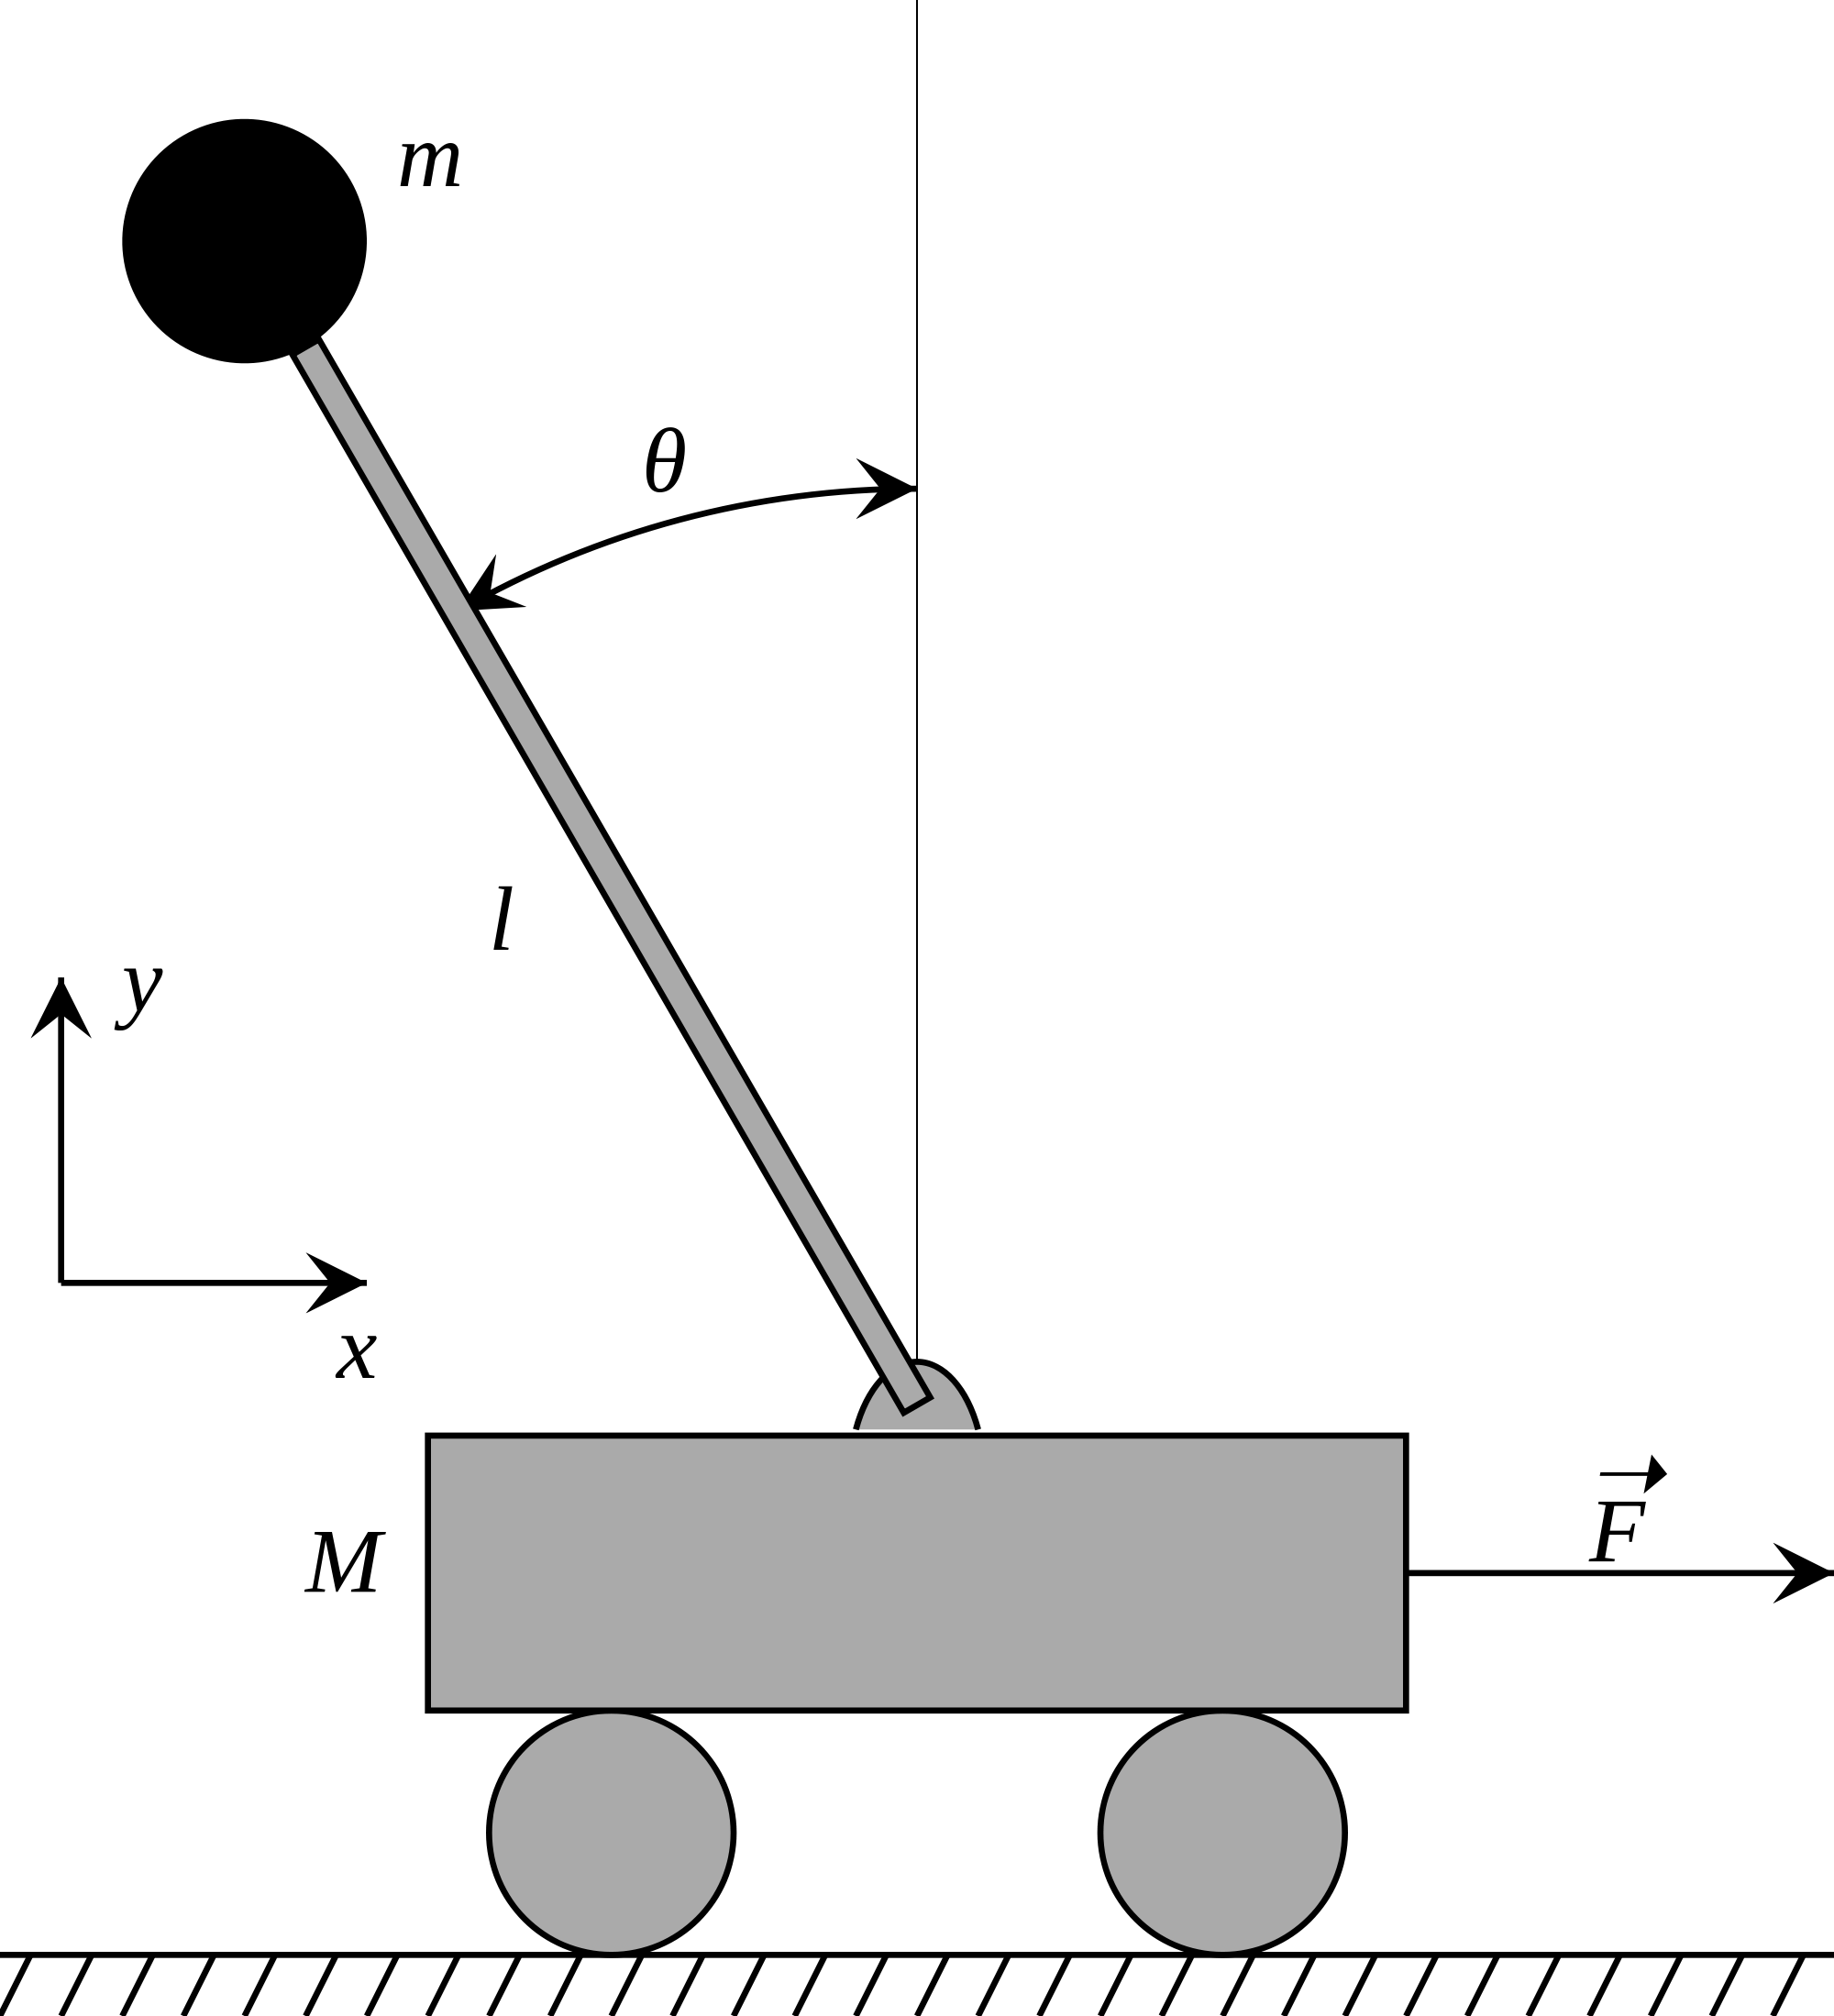
\includegraphics[width=0.5\textwidth]{cart-pole.png}
            \caption{Assume that the mass $m = 0.2kg$, $l = 1.0$, $M = 4.0kg$}
            \label{fig:cartpole}
        \end{figure}
        Describe the equations of motion that govern this system\\
    \textit{Response:} 
        The known variables in the problem are the angle between the pole and the vertical center of mass of the robot ($\theta$), the angular velocity of the pole ($\dot{\theta}$), the position of the cart ($x$), and the velocity of the cart ($\dot{x}$). The known constants are the length of the pole ($l$), the mass at the end of the pole ($m_{p}$), the mass of the cart ($m_{c}$), and the acceleration due to gravity ($g$).
        What we need to know to be able to determine the force needed to keep the pole upright is the angular acceleration ($\ddot{\theta}$):
        $$\ddot{\theta} = \frac{g\sin \theta +\cos \theta\left( \frac{-F-m_{p}l\dot{\theta}^2\sin \theta}{m_{c}+m_{p}} \right)}{l\left( \frac{4}{3}-\frac{m_{p}\cos^2\theta}{m_{c}+m_{p}} \right)}$$
        The acceleration of the cart itself ($\ddot{x}$) is given by:
        $$\ddot{x} = \frac{F + m_{p}l(\dot{\theta}^2\sin \theta-\ddot{\theta}\cos \theta)}{m_{c}+m_{p}}$$

    \part[10] 
        Generate code for a controller that would be able to keep the pole balanced in the air. \\
    \textit{Response:} 
        See the code in our repo. It is the function \texttt{policy()} contained in \texttt{src/MidtermQ4.py}. By running \texttt{src/MidtermQ4.py}, you can see the output as well as our answer to part (c) in this question.
        
    \part[5] 
        What is the maximum angle that my pole can fall to before it cannot recover if max Force $F = 6N $?\\
    \textit{Response:} 
        We wrote some code to test this, and the result was 0.51 radians. See the code in our repo. It is the function \texttt{testMaxTheta()} contained in \texttt{src/MidtermQ4.py}.
\end{parts}
\newpage

\addpoints
\question[20]

    Control and Reinforcement Learning
\noaddpoints
\begin{parts}
    \part[5] 
        Explain three merits and three demerits of using reinforcement learning for mechatronic systems.\\
    \textit{Response:} 
        \textbf{Merits:}
        \begin{enumerate}
            \item After some amount of training, reinforcement learning can generate a perfect model for solving a problem.
            \item Does not need a training dataset to learn (learns from its own rewards and experience instead)
            \item Can solve very complex problems that would take us a long time to solve using math, physics, etc.
        \end{enumerate}
        \textbf{Demerits:}
        \begin{enumerate}
            \item Depends entirely on the previous state to predict the next
            \item Can take an indefinite amount of time to train a model
            \item Needs a lot of data and does a lot of computation
        \end{enumerate}
    \part[5] 
        Draw a diagram for reinforcement learning and controls and contrast the two
    \textit{Response:} 
        \begin{center}
            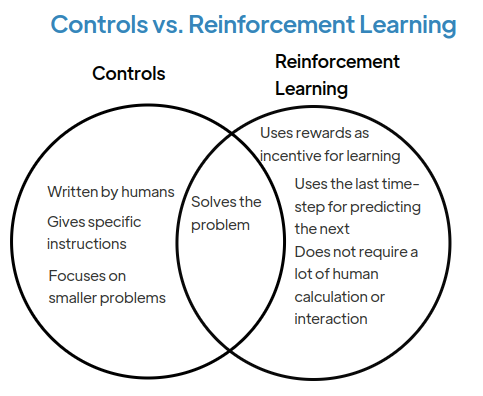
\includegraphics[width=0.6\textwidth]{5-b.png}
        \end{center}
    \part[10] 
         Use OpenAI Gym to create a trained reinforcement learning model for the cart and pole problem (CartPole-v1). 
    
        \url{https://github.com/openai/gym}\\
    
        This tutorial will help you get started with using the OpenAI gym python library. \url{https://blog.paperspace.com/getting-started-with-openai-gym/}\\
    \textit{Response:} 
        Our trained model can be found in our repo by running \texttt{src/MidtermQ5.py}.
    
    \part[10] 
    \textbf{Graduate Question:} Implement this example of a 2D running robot (cheetah) and adapt the code to penalize hip motor movements faster than $\pi \frac{rad}{s}$.  
        \url{https://github.com/openai/gym/blob/master/gym/envs/mujoco/half_cheetah.py} 
        A Virtual Machine that was made with VMWare is available on Canvas for you to use for this question if you have trouble installing Mujoco.

\end{parts}
\newpage



\addpoints
\question[20]
    Human Emotions

\noaddpoints
\begin{parts}

    \part[10] 
        Using the FER library in python, example in the following link:  \url{https://towardsdatascience.com/the-ultimate-guide-to-emotion-recognition-from-facial-expressions-using-python-64e58d4324ff}
        build a system that classifies human emotions and validate on video 1 and 2 from this repository: \url{https://github.com/rjrahul24/ai-with-python-series/tree/main/07.%20Emotion%20Recognition%20using%20Live%20Video}
        Generate plots of predicted emotions over time for both videos.

    \part[5]
        Do the same as the above with a video feed from your webcam. Set your software up to allow video feed or a pre-recorded video. (In essence, make faces at yourself and make sure that your service works). Submit a short faces-recording along with the script that can read live webcam streams. 
    
    \part[5] 
        What are the logical applications of this tool for an autonomous robot? What are the ethical and legal consequences of fielding a system that makes decisions based on this tool?

    \part[10]
        \textbf{Graduate Question:} Set up a service that allows 2 or more faces to be processed at once.
\end{parts}

\textit{Response:}

\begin{parts}
	\part
	View the provided \verb|MidtermQ6.py| script for the code that generated these images. It has a help menu and a friendly interface to work with.
	\begin{figure}[H]
	\centering
		\begin{minipage}[b]{\textwidth}
			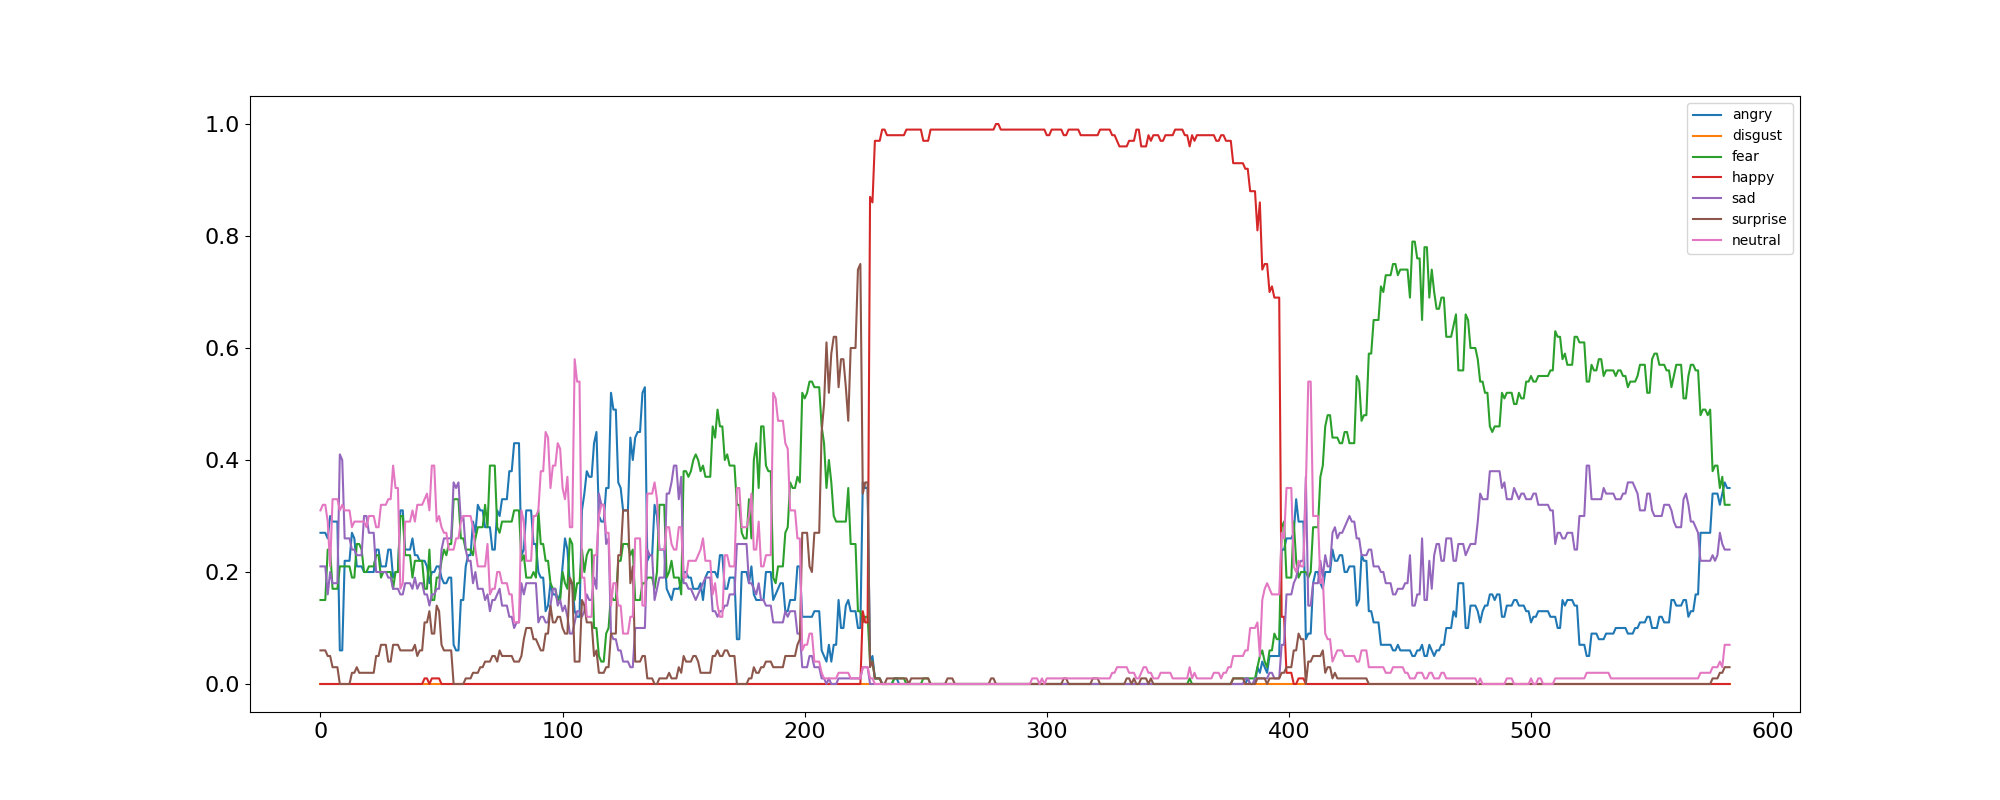
\includegraphics[width=\textwidth]{Video_One-plot.png}
			\caption{Video One Plot.}
		\end{minipage}

		\hfill

		\begin{minipage}[b]{\textwidth}
			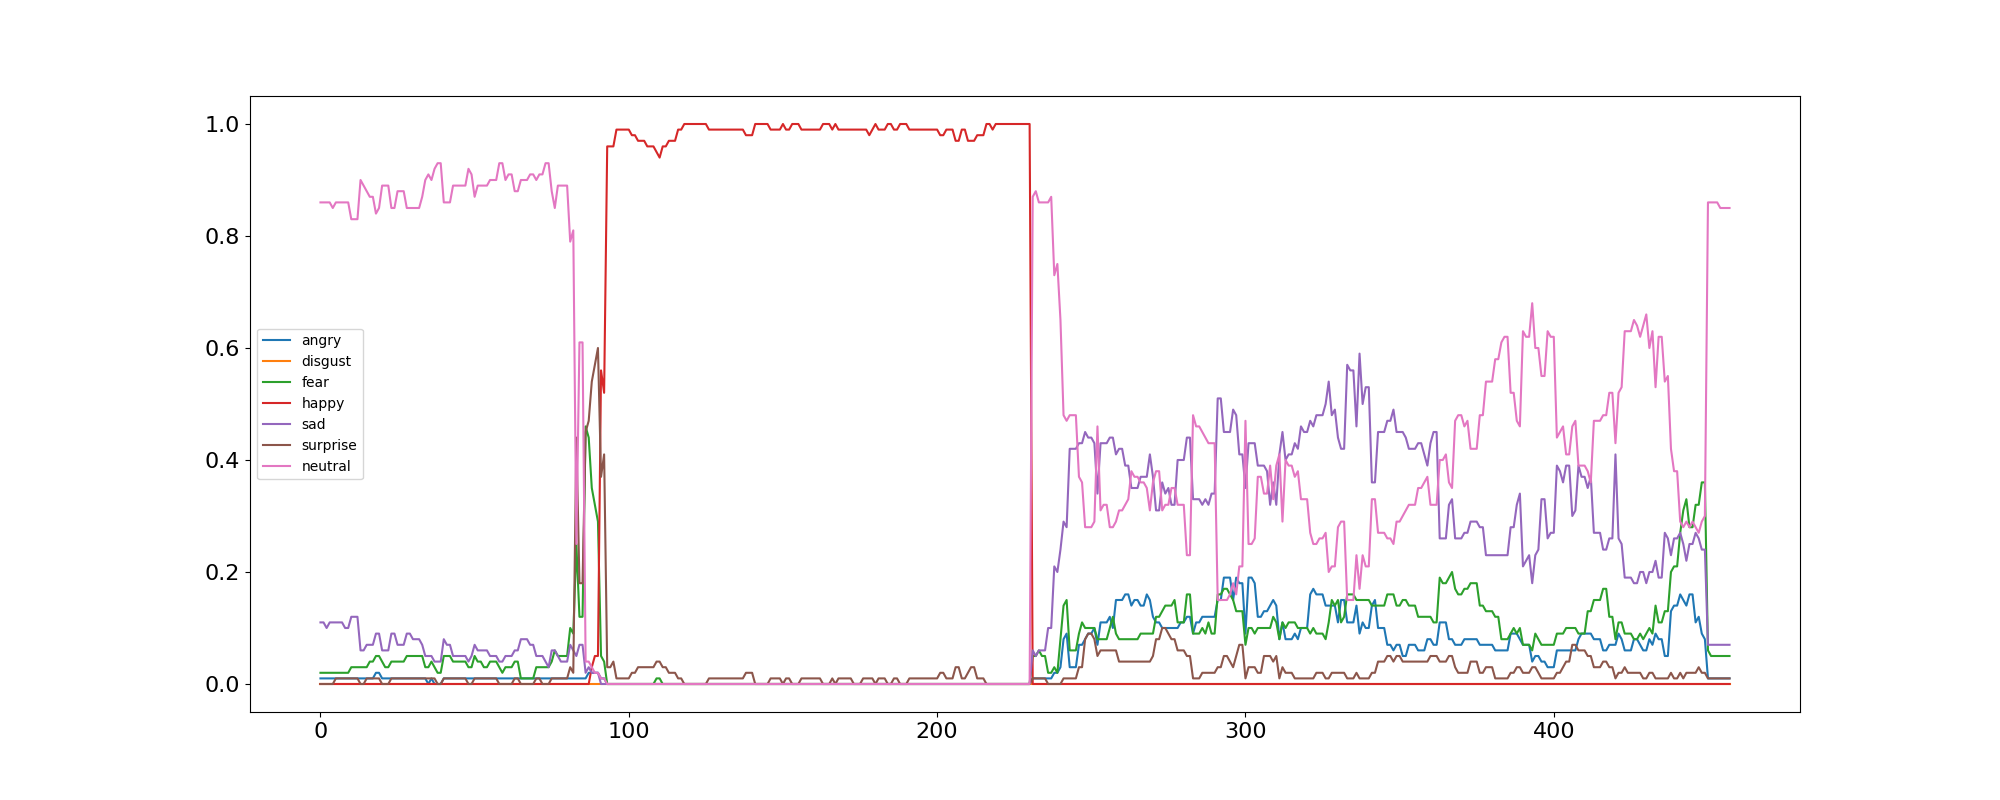
\includegraphics[width=\textwidth]{Video_Two-plot.png}
			\caption{Video Two Plot.}
		\end{minipage}
	\end{figure}

	\part 

		See the included python script and video \verb|my_example.webm| in the provided videos for the source of this plot.

		\begin{figure}[H]
		\centering
		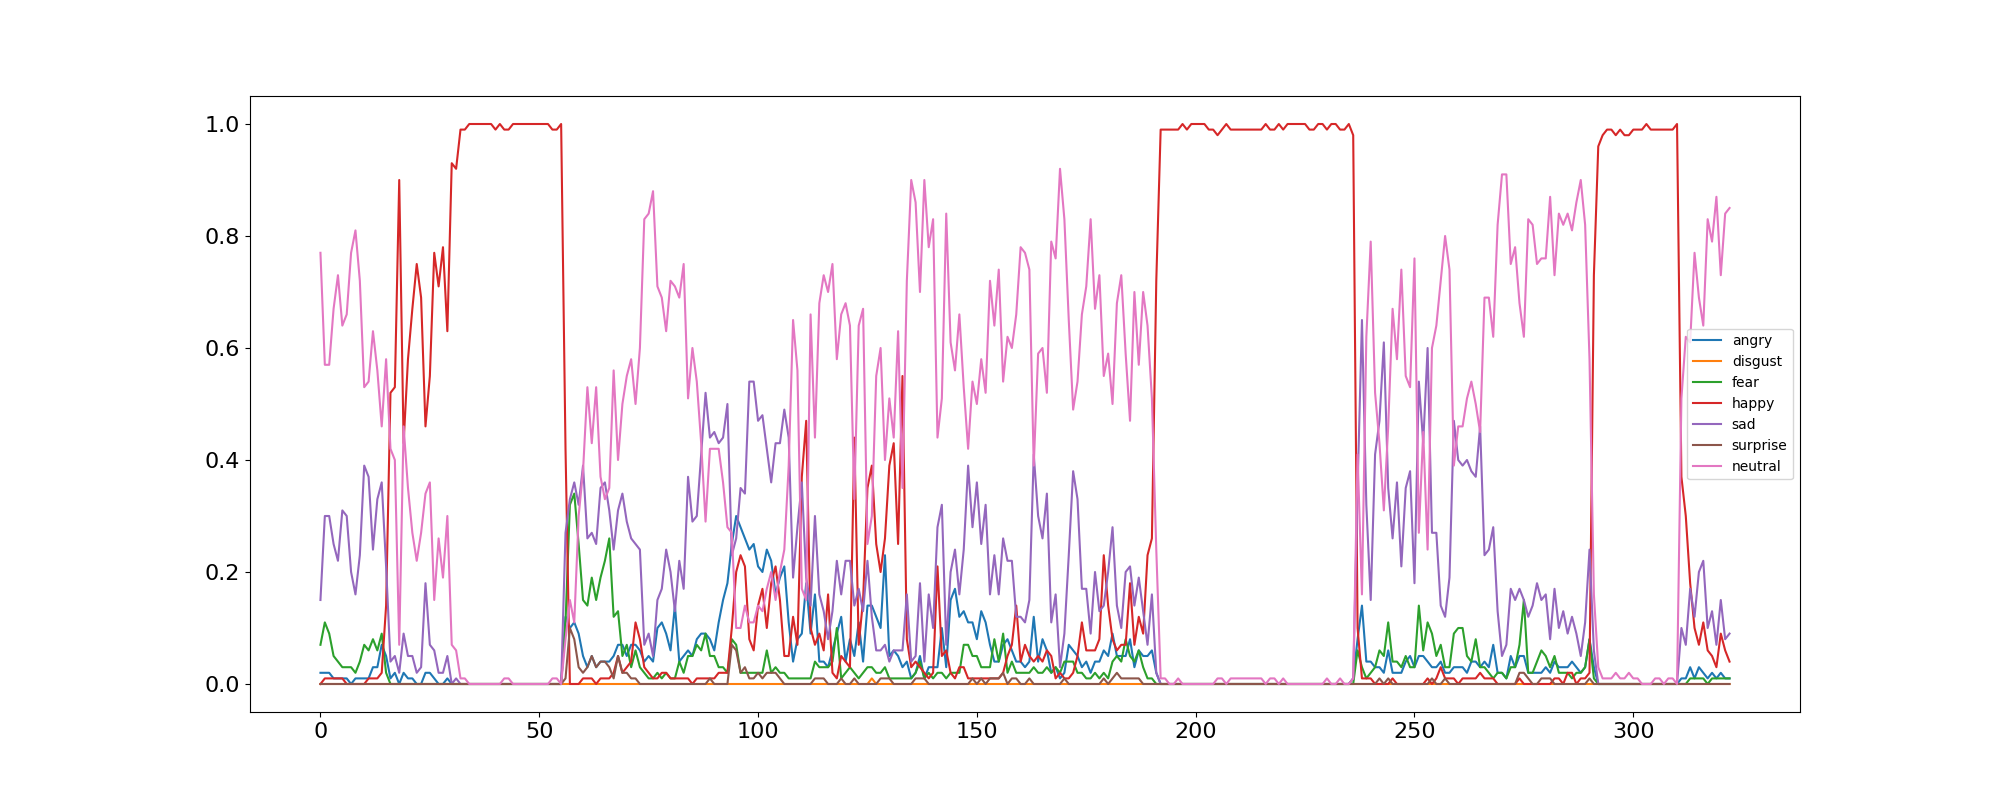
\includegraphics[width=\textwidth]{my_example-plot.png}
		\caption{my\_example.webm Plot.}
		\end{figure}

	\part
	This tool can pretty obviously be applied to help a robot understand what a human is feeling, and change it's behavior to match the human's mood. This can be pretty problematic immediately, for several reasons. Any time we're using human facial imagery in robotics, we need to think about privacy concerns and law enforcement. Will the police try to get access to our footage? Is that ethical? This is an issue that our society is still grappling with, especially after seeing facial imagery being used so prevalently against protestors in Hong Kong.

	Additionally, can we trust a robot to behave correctly given particular facial expressions? We need to know that our facial recognition algorithm is reliable. Humans are a widely varied species, and historically such models are not always trained in a way that represents the broad intersectionality of our people. Can the algorithm work consistently with different face shapes, colors, and other characteristics? If not, our tool could end up causing more issues than it solves.

	\part

	Again, reference \verb|MidtermQ6.py| for this. When invoked with the \verb|-t| option, the script will execute with support for two faces in the video, and generate a plot for each of them.
	
	\begin{figure}[H]
	\centering
		\begin{minipage}[b]{\textwidth}
			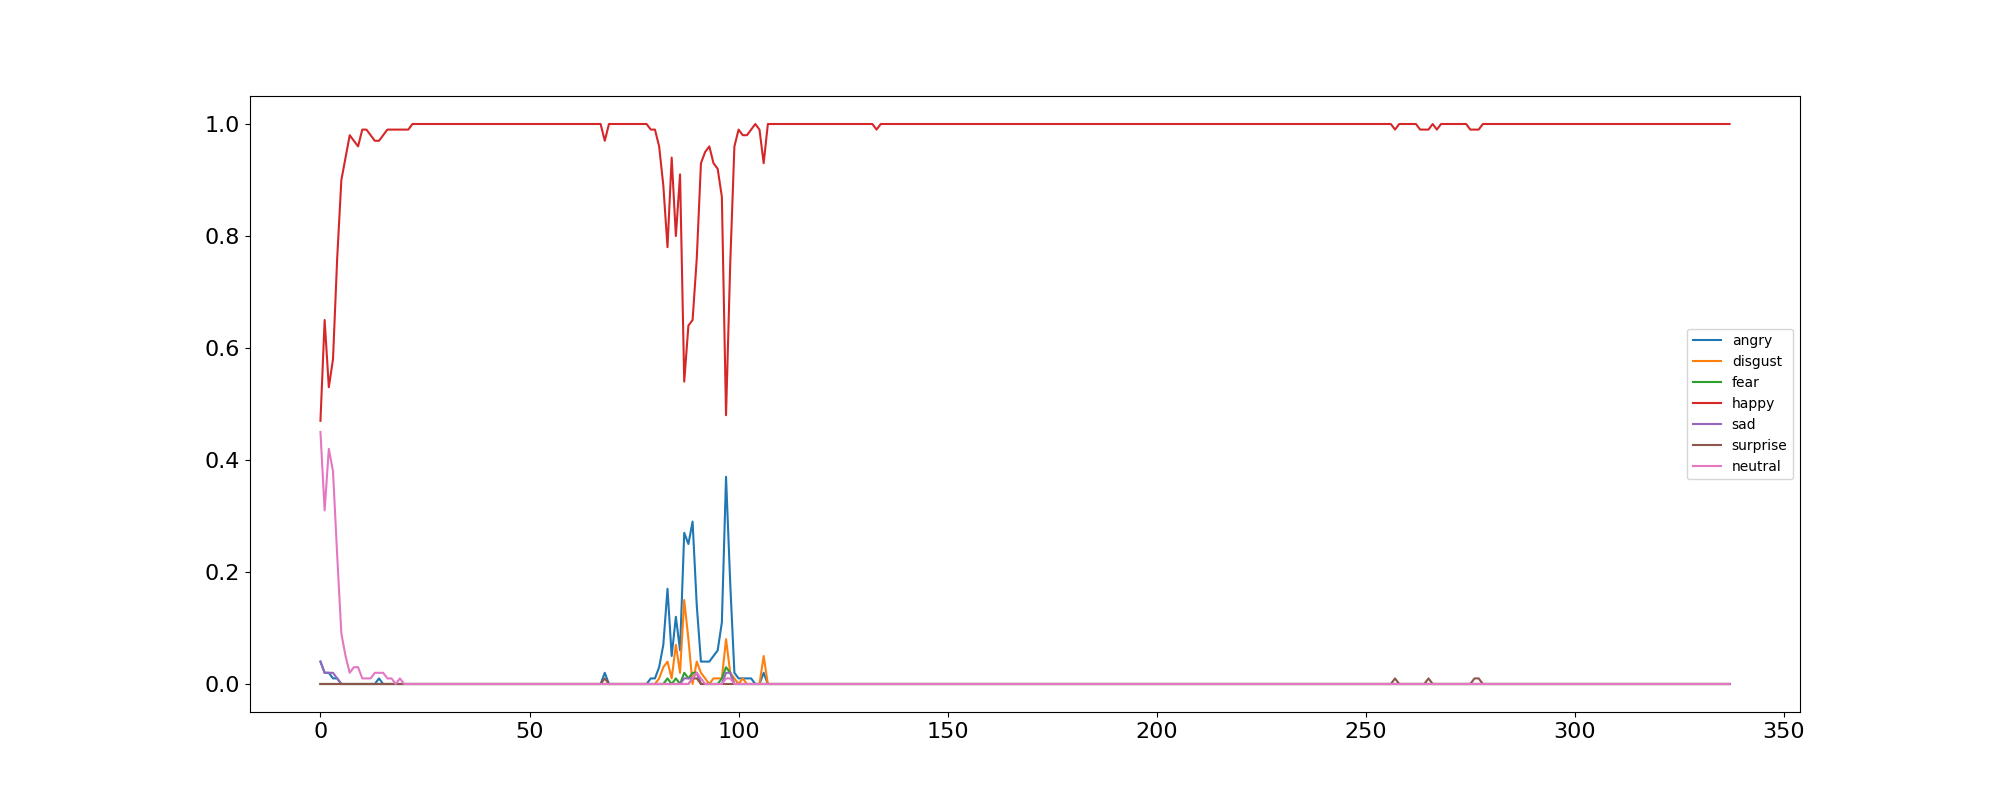
\includegraphics[width=\textwidth]{two_test-face1-plot.png}
			\caption{two\_test.mp4 First Face Plot.}
		\end{minipage}

		\hfill

		\begin{minipage}[b]{\textwidth}
			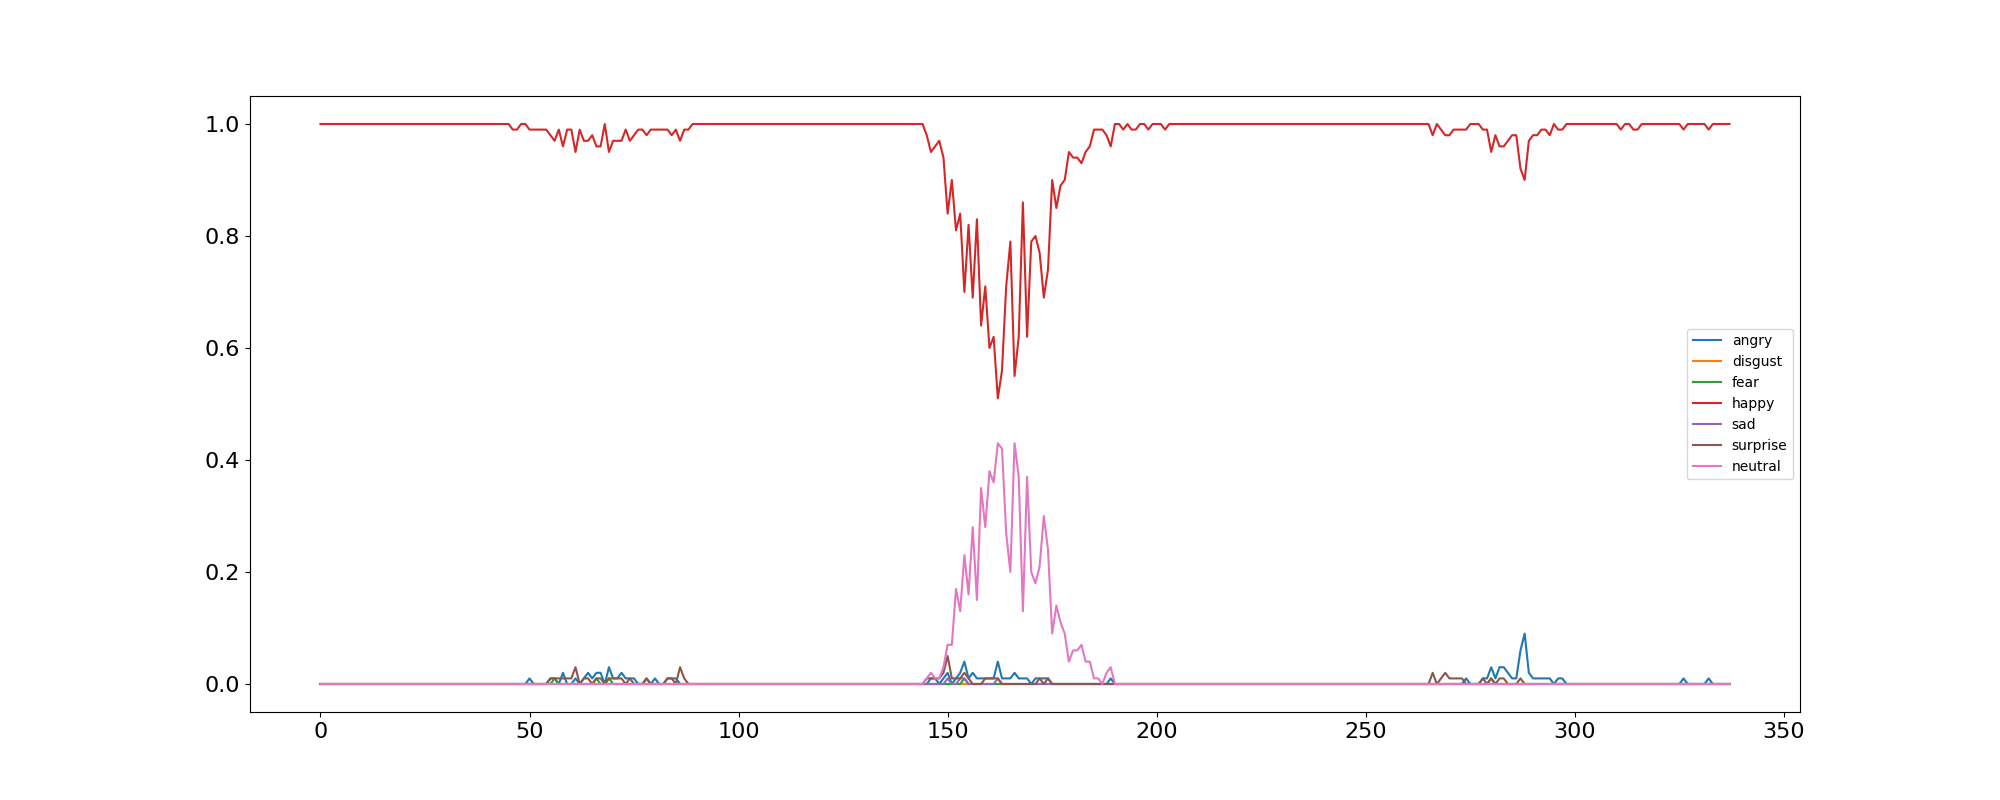
\includegraphics[width=\textwidth]{two_test-face2-plot.png}
			\caption{two\_test.mp4 Second Face Plot.}
		\end{minipage}
	\end{figure}


\end{parts}
\newpage

\addpoints
\question[20]
    Motion Planning

\noaddpoints
\begin{parts}

    \part[20] 
        Implement an A* based planner (an example is found here: \url{https://medium.com/@nicholas.w.swift/easy-a-star-pathfinding-7e6689c7f7b2}) and compare it's results with the Djikstra, A-Star, RRT-Star, Bi-Directional A-Star, and the Breadth First Search Planners from this github. \url{https://github.com/AtsushiSakai/PythonRobotics/tree/master/PathPlanning}. 
        Create a table comparing the average cost of the path found over 10 iterations along with the time to convergence. 
    
        After you have implemented your planner and compared it answer the below questions. 
        \begin{itemize}
            \item Which planner provided a path with the lowest cost on average?
            \item Which one found a path the fastest on average? 
            \item After comparing your planner to these five other ones is there anything you would change in your planner to help it converge faster or find a path with a better cost?
            \item Which planner appears to be the best overall? Which planner would you use for a robot in a complex environment? 
        \end{itemize}
    
        % Could we just make the designing and building a planner the most important part of this? 
        % \part[10] 
            % Implement a skid-steer (4 wheel) vehicle model for a robot 33 inches wide, by 40 inches long for the planner that you chose.
    
    \part[10]
        \textbf{Graduate Question:} 
        Implement a skid-steer (4 wheel) vehicle model for a robot 33 inches wide, by 40 inches long for the Hybrid A* algorithm. Change the scenario so both your A* and Hybrid A* have the same obstacle field. Compare and contrast the final trajectories, graph these. Write what the algorithmic differences are between the two planners and how the kinematics are used to constrain the Hybrid A*.
        
        % Take your A* algorithm and change it to be a sampling-based planner. To do this, rather than working in a grid-based environment, we will now be in continuous space with each sample taking you to a new position. Use a skid-steer vehicle model to sample from.

\end{parts}
\textit{Response:} 
Code for this problem is found in MidtermQ7.py Please note that we gave credit to the author of the Implemented A* algorithm.
    \\
    \begin{center}
        Average Time and Cost of Algorithms
        
        \begin{tabular}{||c c c c c c||} 
             \hline
             & Dijkstra & Bi-Directional & RRT* & Other A* & Implemented A* \\ [0.5ex] 
             \hline\hline
             Avg Time: & 0.014s & 0.024s & 2.437s & 0.030s & 0.002s \\ 
             \hline
             Avg Cost: & 59.60 & 61.36 & 71.30 & 59.60 & 40.63 \\ [1ex] 
             \hline
        \end{tabular}
    \end{center}
\newpage
\textit{Response Continued:}

    \begin{itemize}
            \item Lowest cost: Our implemented A*
            \item Fastest: Our implemented A*
            \item Changes to our implemented A*: I noticed that the original code was not allowing diagonal traversal. It appears that this issue was fixed in a later implementation. Before using the updated implementation our implementation was the slowest and the most costly. However, once we started using diagonal pathing it became the best one out of the bunch.
            \item Best Overall: Our implemented A*. Without knowing what complex environment our robot would be in, we feel like the A* would be best based on our findings. The maze we used for these averages is small, so there may be a case that the Bi-Directional could be more useful in a more complex environment. However, given the information we have, our implemented A* algorithm seems like the best option.
    \end{itemize}
\newpage

\addpoints
\question[20]
    Object Detection (Please put the classified images as part of your submission)

\noaddpoints
\begin{parts}
    % Carter will solve this problem Yay! Agriculture might be great
    \part[5] 
        Classify the first 10 pictures in \url{https://github.com/ravirajsinh45/Crop_and_weed_detection} using any image classification algorithm.
    
    \part[5] 
        Implement Yolo and do the same, what are the differences. 
    
    \part[10] 
        Using transfer learning, pick an image classification algorithm and retrain it to learn to detect a new object of interest.

    \part[10]
        \textbf{Graduate Question:} Implement Detectron (\url{https://github.com/facebookresearch/Detectron}) and  test the image segmentation of the objects you are interested in. Give metrics on relative segmentation/classification quality comparing: Mask R-CNN, faster R-CNN, and RetinaNet.

\end{parts}

\textit{Response:}
\begin{parts}

	\part
    We implemented a MobileNet-SSD v3 model to predict the 10 plant images in the sample data set. This model was not trained on plant identification, so the predictions are very inaccurate. 
    
        \begin{figure}[H]
			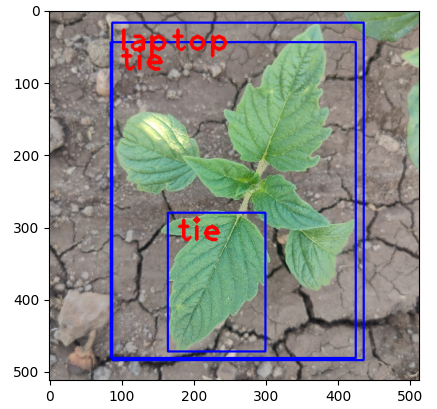
\includegraphics[width=\textwidth]{images-SSD/plant1.png}
			\caption{SSDpredictionPlant1.png}
		\end{figure}

		\hfill

		\begin{figure}[H]
			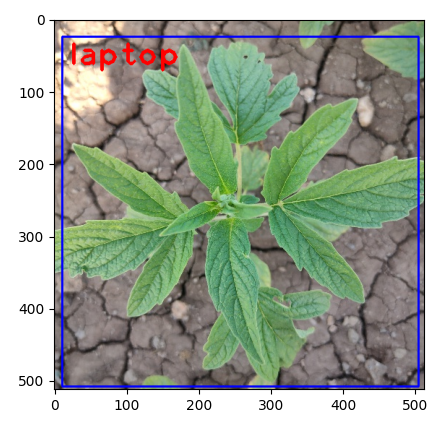
\includegraphics[width=\textwidth]{images-SSD/plant2.png}
			\caption{SSDpredictionPlant2.png}
		\end{figure}

		\hfill

		\begin{figure}[H]
			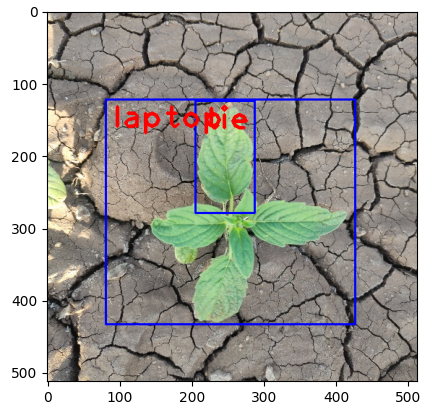
\includegraphics[width=\textwidth]{images-SSD/plant3.png}
			\caption{SSDpredictionPlant3.png}
		\end{figure}

		\hfill

		\begin{figure}[H]
			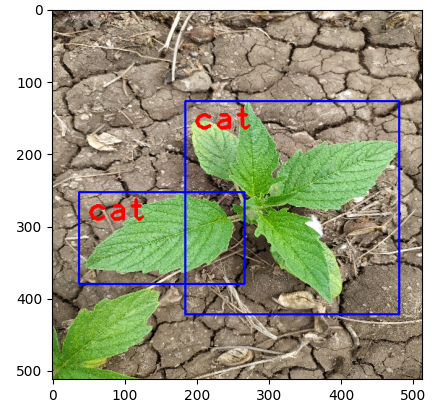
\includegraphics[width=\textwidth]{images-SSD/plant4.png}
			\caption{SSDpredictionPlant4.png}
		\end{figure}

		\hfill

		\begin{figure}[H]
			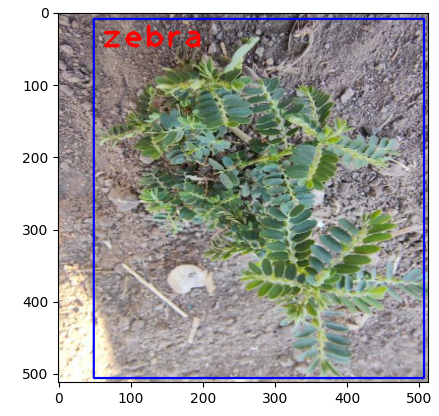
\includegraphics[width=\textwidth]{images-SSD/plant5.png}
			\caption{SSDpredictionPlant5.png}
		\end{figure}

		\hfill

		\begin{figure}[H]
			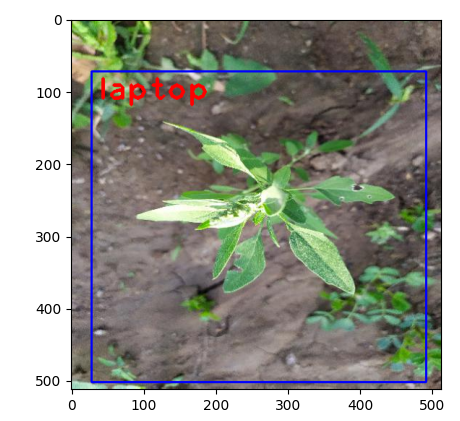
\includegraphics[width=\textwidth]{images-SSD/plant6.png}
			\caption{SSDpredictionPlant6.png}
		\end{figure}

		\hfill

		\begin{figure}[H]
			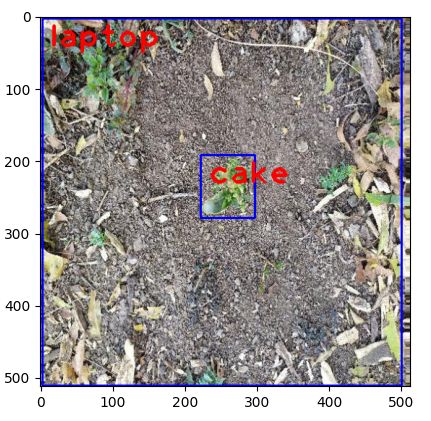
\includegraphics[width=\textwidth]{images-SSD/plant7.png}
			\caption{SSDpredictionPlant7.png}
		\end{figure}

		\hfill

		\begin{figure}[H]
			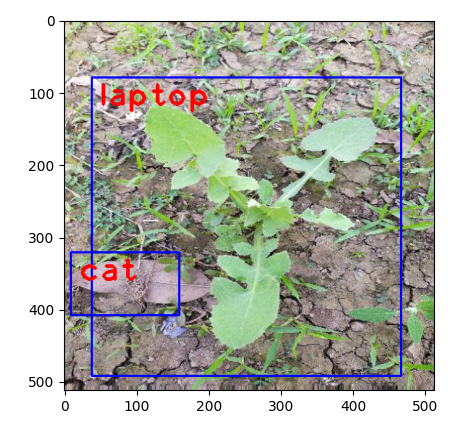
\includegraphics[width=\textwidth]{images-SSD/plant8.png}
			\caption{SSDpredictionPlant8.png}
		\end{figure}

		\hfill

		\begin{figure}[H]
			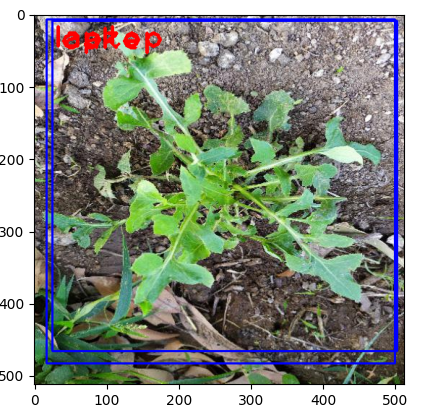
\includegraphics[width=\textwidth]{images-SSD/plant10.png}
			\caption{SSDpredictionPlant10.png}
		\end{figure}

		\hfill
    
	\part
	We were able to implement YOLO using the method linked to the sample data set. It wasn't perfectly accurate, but we did get bounding boxes around the test images it recognized well. Here are the classified test images I generated: 

		\begin{figure}[H]
			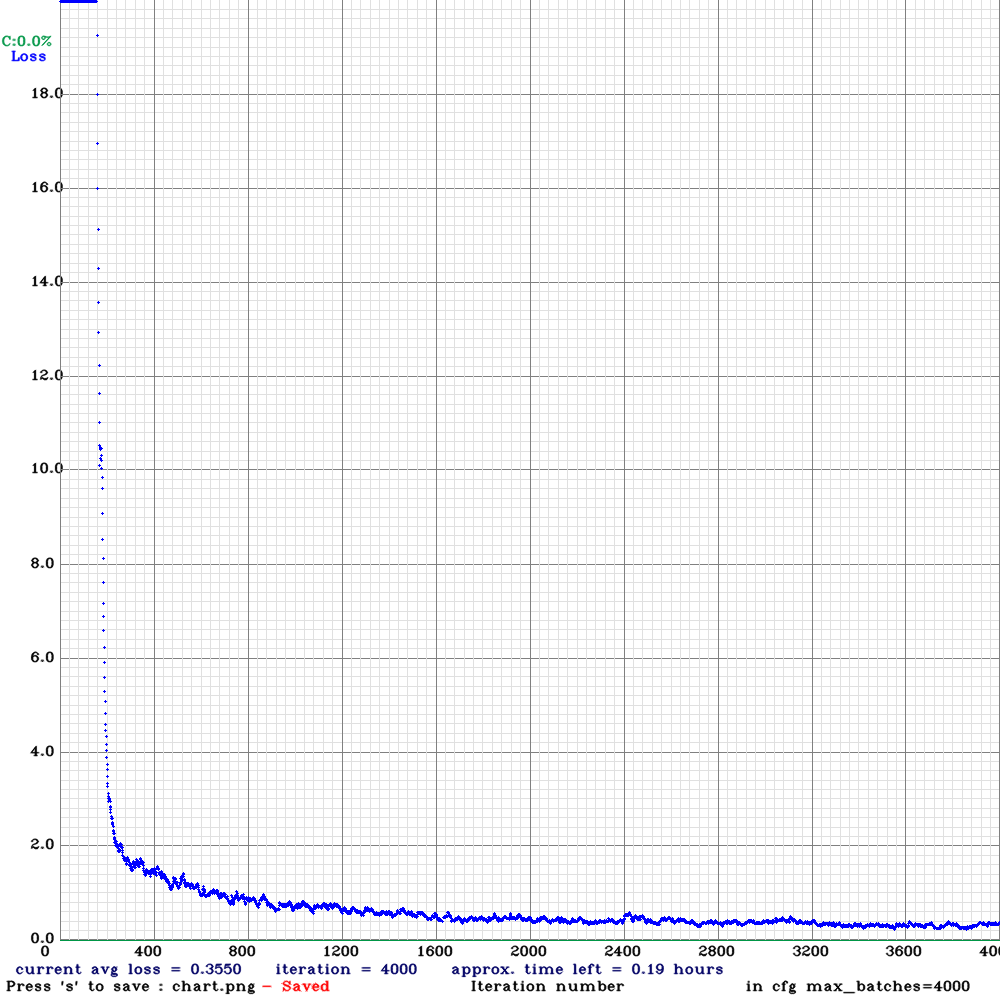
\includegraphics[width=\textwidth]{images-yolo/chart_crop_weed.png}
			\caption{YOLOv4 Training chart.}
		\end{figure}

		\hfill

		\begin{figure}[H]
			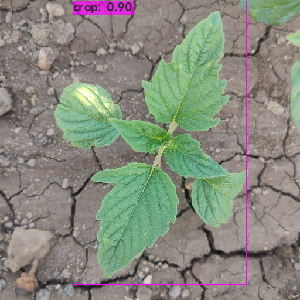
\includegraphics[width=\textwidth]{images-yolo/prediction_crop_1.png}
			\caption{prediction\_crop\_1.png}
		\end{figure}

		\hfill

		\begin{figure}[H]
			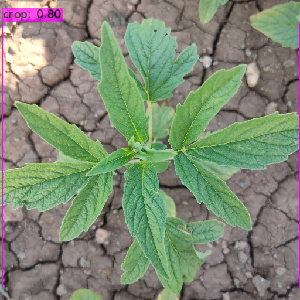
\includegraphics[width=\textwidth]{images-yolo/prediction_crop_2.png}
			\caption{prediction\_crop\_2.png}
		\end{figure}

		\hfill

		\begin{figure}[H]
			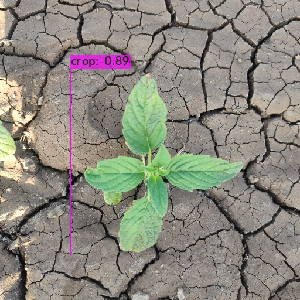
\includegraphics[width=\textwidth]{images-yolo/prediction_crop_3.png}
			\caption{prediction\_crop\_3.png}
		\end{figure}

		\hfill

		\begin{figure}[H]
			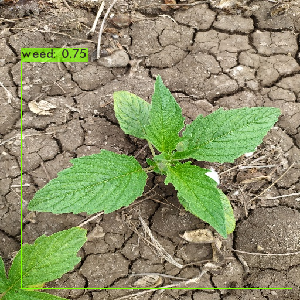
\includegraphics[width=\textwidth]{images-yolo/prediction_crop_4.png}
			\caption{prediction\_crop\_4.png}
		\end{figure}

		\hfill

		\begin{figure}[H]
			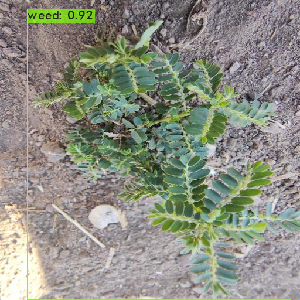
\includegraphics[width=\textwidth]{images-yolo/prediction_weed_1.png}
			\caption{prediction\_weed\_1.png}
		\end{figure}

		\hfill

		\begin{figure}[H]
			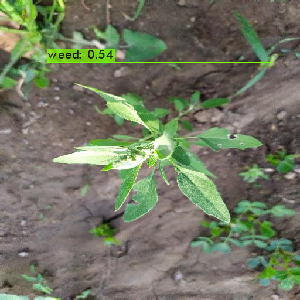
\includegraphics[width=\textwidth]{images-yolo/prediction_weed_2.png}
			\caption{prediction\_weed\_2.png}
		\end{figure}

		\hfill

		\begin{figure}[H]
			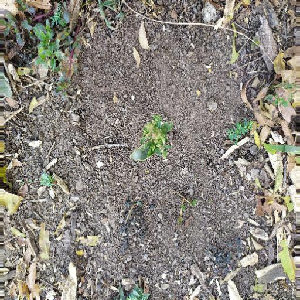
\includegraphics[width=\textwidth]{images-yolo/prediction_weed_3.png}
			\caption{prediction\_weed\_3.png}
		\end{figure}

		\hfill

		\begin{figure}[H]
			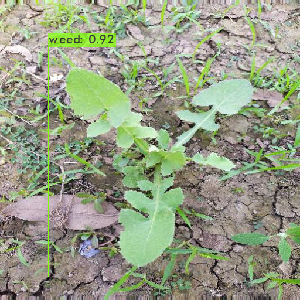
\includegraphics[width=\textwidth]{images-yolo/prediction_weed_4.png}
			\caption{prediction\_weed\_4.png}
		\end{figure}

		\hfill

		\begin{figure}[H]
			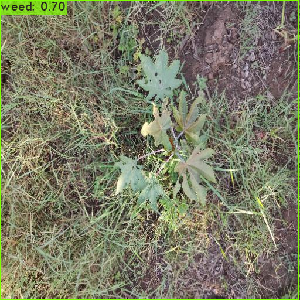
\includegraphics[width=\textwidth]{images-yolo/prediction_weed_5.png}
			\caption{prediction\_weed\_5.png}
		\end{figure}

		\hfill

		\begin{figure}[H]
			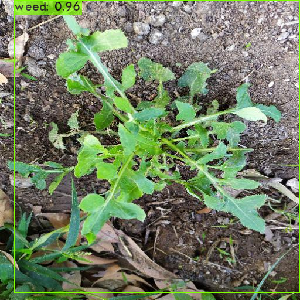
\includegraphics[width=\textwidth]{images-yolo/prediction_weed_6.png}
			\caption{prediction\_weed\_6.png}
		\end{figure}


	\part
	We attempted to use Resonant50 for transfer learning, using TensorFlow and Keras. The included scripts can be found in the provided python files \verb|MidtermQ8-train-resnet.py| and \verb|MidtermQ8-teset-resnet.py|, with the sample dataset in \verb|Q8-crop-weed-dataset| and the generated model in \verb|model_karas/|. This model trained a lot faster than the other ones did, since we were able to leverage mostly pre-trained model. However, we were not able to get this model to successfully classify images in the allotted time- it just produces "crop" results for every image tested. 

\end{parts}

%%%% Removed question 9 due to time constraints
% \newpage
% \addpoints
% \question[20]
%     Full Circle - Car planning in a complex environment

% \noaddpoints
% \begin{parts}

%     \part[5]
%         A pedestrian suddenly begins to walk in front of the moving vehicle ($11 m/s$).  The pedestrian is 20 meters in front of the car. What commands will the car need to receive to stop before it hits the pedestrian? Plot the velocity, position, and commanded inputs. 
%     \part[5] 
%         Assume that your vehicle can only decelerate at $4.2 m/s^2$ (max). If there is an open lane to your left or right, generate a new stopping trajectory. Plot the velocity, position, and commanded inputs. 
%     \part[5] 
%         A New vehicle pulls out into the road 15 meters ahead of you and speeds up to $11 m/s$. Design a trajectory to pass on the left if your vehicle is moving at $13 m/s$. Plot the velocity, position, and commanded inputs. 
%     \part[5]
%         As you are passing the vehicle (where you begin to overlap), it speeds up to $13 m/s$. Compute a new passing trajectory if you are willing to accelerate to $14 m/s$, how much time will you be in a "Passing" maneuver? Plot the velocity, position, and commanded inputs. 

    % \part[10] \textbf{Graduate Question:}
    %     Traffic aware navigation - Your vehicle is stopped at an intersection making a left turn (yay). You are able to accelerate at 12 mph/s
    
    % \part[10]
    %     Using the autonomous driving dataset \url{https://www.nuscenes.org/nuimages#data-collection} combine sensors to build a spatial map of objects. Using Yolo and Python, build a visualization of all identified objects and their relative positions. 
        
    % \part[10]
    %     Integrate the CAN information using the nuscenes devkit \url{https://github.com/nutonomy/nuscenes-devkit}. 
    %     \begin{itemize}
            
        %     \part[10] \textbf{Graduate Question:} (Choose one) 
        %     Power aware navigation - Generate a power model of the vehicle to predict the power cost of maneuvers (hint, should be highly correlated with acceleration), and generate a route that optimizes the energy. 
            
        % \end{itemize}
        
% \end{parts}
\newpage

\addpoints
\question[20]
    Ethics of Robotics - Open Ended Questions

\noaddpoints
\begin{parts}
    
    \part[5] 
        Many people (particularly those in the robotics industry) believe that robotics is purely within the purview of technical development and should not have any ethical considerations. What do you feel can be a merit or demerit to this way of thinking?
    
    \part[5] 
        Isaac Asimov listed 3 laws of robotics, comment on the algorithmic complexity of implementing these into working intelligence. Define a scenario and write Psuedo code to implement these rules. 
    
    \part[5] 
        In the event of an autonomous system causing harm or damages, who is responsible? Read and comment on the following two documents: \url{https://www.callahan-law.com/articles-and-expert-advice/when-an-autonomous-vehicle-hits-a-pedestrian-who-is-responsible/} and \url{https://en.wikipedia.org/wiki/Self-driving_car_liability}
    
    \part[5] 
        What laws may be helpful for regulating or controlling autonomous systems? What drawbacks will this potentially have?

\end{parts}

\textit{Response:}

\begin{parts}
    
    \part A merit to this way of thinking is the rate of development. If you look at robots as machines and nothing more, then the tests you perform on them should not matter ethically (towards the robot). This allows for faster testing and overall production. There are many videos that depict testing as being rough and mean towards the robots, but they are necessary tests for limit testing. Until we have a robot that is verifiable conscious, I don't think that ethics should be a consideration.
    
    \part
    \begin{enumerate}
        \item \textbf{First law:} A robot may not injure a human being or, through inaction, allow a human being to come to harm. This law has a lot of complexity. Having the robot not harm the human is difficult, but always being on the lookout for harm and not allowing said harm to occur is much harder. How does a robot even predict EVERY possible way for a human to get hurt? And then how would it know how 
    	to solve such situations?
        \item \textbf{Second law:} A robot must obey the orders given it by human beings except where such orders would conflict with the First Law. This law sounds a lot simpler at surface level. I do think it is more simple than the First Law. However, what if it is given two conflicting orders? How does it resolve those orders? How does it think through a paradoxical order without getting stuck? When we think about these questions we can see that the second law is still very complex.
        \item \textbf{Third law:} A robot must protect its own existence as long as such protection does not conflict with the First or Second Law. Because the robot needs to be constantly thinking about the first and second law, this makes the third law complex. It would need to verify that any action it took to protect itself does not violate the two previous laws.
        \newpage
        \item \textbf{Scenario:} A human-like robot is walking from the grocery store to get cat food for its owner's cat. It sees a man fall on the ground dangerously close to traffic. It stops following the Second law, to uphold the first law. It rushes to the man and positions itself in the street in front of traffic, ignoring the third law to uphold the first. However, it must only do this if it deems likely that a collision with the robot will not harm a driver. Having deemed this action safe, it goes into the street and stops traffic. Once that danger has been avoided, it continues with its task and upholds the second law.
        \item \textbf{Psuedo Code:}
            \begin{verbatim}
    while(powered on):
        			Create Task: Look for humans
        		    {
        			    Scan environment
        			        Check every object
        			        If object is human:
        			            Classify human
        			            Classify threat level
        			            Store human in map/memory
        		    }
        		    Create Task: Listen for command
        		    {
        		    If (command is issued):
        		        Create Task: Perform command
        		    }
        		    Create Task: Protect Self
        		    {
        			    Scan environment
        			        If object is threat to self:
        			            avoid object
        			                if avoiding causes harm to human:
        			                    abort avoid
        		    }
        		    
        		    If (human is found and in danger):
        		        Stop Task: Perform command
        		        Stop Task: Protect Self
        		        If (human no longer in danger):
        		            Start Task: Perform command
        		            Start Task: Protect Self

            \end{verbatim}

    \end{enumerate}
    \newpage
    \part Who is responsible for harm done by autonomous vehicles? It's a massive 'depends'. In the article "When an autonomous vehicle hits a pedestrian, who is responsible?" It talks about how there was a driver in the car at the time of the accident, but they were not paying attention when the accident occurred. Even though the car may be autonomous, I think that the human driver is ultimately responsible if they are in the car at the drivers seat.
	In the Wikipedia article it talked about many different types of responsibility. It's argued that if the car is totally self reliant, and an accident occurs with no human in the drivers seat, it is the manufacturers concern. If the vehicle is physically faulty, that's a manufacturers problem. Other ideas is that the person who issued the command is responsible. The fear is that there is no way to predict all accidents, so manufacturers could be sued to oblivion if it is their sole responsibility. We are trying to get to a place where responsibility can be shared, so that the burden doesn't rest all on one party.
    
    \part
    \begin{enumerate}
        \item You cannot be in a self driving car unless you have a valid drivers licence, or you are with someone who does. The person with a driver license is responsible for paying attention to the road to prevent unforeseen accidents. \\
        
        Drawbacks: Not as many people can use these self driving vehicles. It also removes some usefulness of the self driving car. Not paying attention while its driving is a big selling point. \\
        
        \item All autonomous systems must be under some form of human supervision. \\
        
        Drawbacks: If it needs to be supervised, is it autonomous? This law may defeat the purpose of some systems and their usefulness. It also means that we will need to come up with effective ways for one person to monitor many systems if this law is to be effective.
    \end{enumerate}
\end{parts}




% \question[10]
% In no more than two sentences, explain the difference between RRT* and A*.
% % \makeemptybox{2in}

% \question[10]
% Write the psuedo code for the Djikstra's algorithm and explain how it searches a space and finds the optimal path
% % \makeemptybox{\fill}

% \question[10]
% Write the psuedo code for the RRT* algorithm and explain how the search can be  guided

% \question[15]
% \noaddpoints
% Understanding key algorithms
% \begin{parts}
% \part[5] List two unique features of the RRT*, A*, and Djikstra's algorithm
% \part[5] Which algorithm is best suited for an holonomic ground robot with few known obstacles? (Why? What are your assumptions?)
% \part[5] Which algorithm is best suited for navigation autonomy on a field combat tank? (Why? What are your assumptions?)
% \end{parts}


% \addpoints
% \question[20]

% Robot Arms

% \noaddpoints
% \begin{parts}



% \part[5] 
% \begin{figure}
% \centering
% 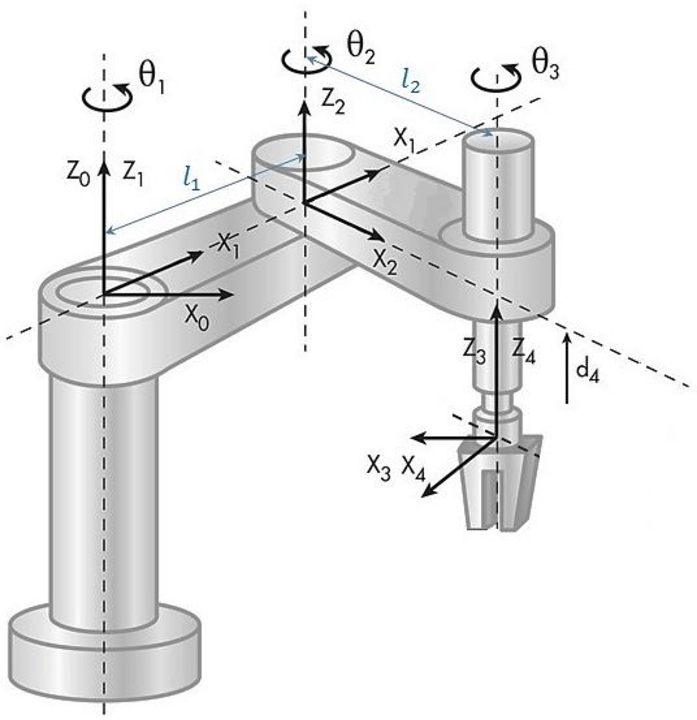
\includegraphics[width=0.5\textwidth]{SCARA-robot-of-4-gdl-Source-Our-elaboration.png}
% \caption{SCARA type manipulator. }
% \end{figure}

% What is the workspace volume for this robot?. (Draw a picture of it as well)
% \part[5] Write the DH parameters and forward kinematics for this robot 
% \part[10] Compute the inverse kinematics to get the robot to pick up an object at x=1.2, y=0.8, z=0.5

% \end{parts}
% \newpage

% You are tasked with surveying a remote agricultural area in Cote d'Ivoire which produces cocoa beans for top chocolate makers (yay chocolate!). Because of the costs of operation in this region of the world, you have been tasked with getting a robot to move from a base-station to survey a small patch of cocoa trees and estimate crop yeilds. 

% \noaddpoints
% \begin{parts}
% \part[5] What is the state space of the problem? What are the critical pieces of information that you feel is relevant to solving the problem? Are there any assumptions you are making in being able to access this information? Write this as a list, ie: State = ['something1', 'something2', ect.], assumptions = ['none', 'heroic assumption about amazing sensor', ect.]

% \part[10] Write your cost function? Does it have units? (If yes, what are they?) What are you penalizing/rewarding? Write this in the form of: Cost = <function>

% \part[10] What is a good heuristic function that can estimate your cost to accomplish this objective? (Note that this should be in the same units as your cost function.) What are the drawbacks and simplifications this function is making?

% \part[15] 
% What would your search algorithm look like? Illustrate the logic your system would follow to make a crop yeild estimate. (Draw a diagram of a few trees, where would your robot go first, how does your cost and heuristic fit together?) How much would you trust this information in making decisions about moving labor and resources here?


% \end{parts}

% \fillwithdottedlines{8em}

\end{questions}
\end{document}

